%  Typ dokumentu - článek, prezentace aj.
\documentclass[english]{article}

%  Nastaví vstupní a výstupní kódování znaků (encoding) a lokalizace
\usepackage[T1]{fontenc}
\usepackage[utf8]{inputenc}
\usepackage[english,czech]{babel}
\usepackage{icomma}
\usepackage{lmodern}

%  Formát papíru a odsazení od jeho okrajů
\usepackage[letterpaper]{geometry}
\geometry{verbose,tmargin=1.5cm,bmargin=2cm,lmargin=2cm,rmargin=2cm}

%  Umožňuje pracovat s grafikou
\usepackage{graphicx}

%  Automaticky odsadí i první paragraf v každé sekci
\usepackage{indentfirst}

%  Umožňuje rozdělovat obsah na více sloupců
\usepackage{multicol}

%  Umožňuje používat hypertextové odkazy, nastavuje jejich barvu a
%  vlastnosti
\usepackage[unicode]{hyperref}
\hypersetup{
colorlinks=true, citecolor=blue, filecolor=blue, linkcolor=blue,
urlcolor=blue
}

%  Umožnění odstranění italiky u jednotek
\newcommand{\unit}[1]{\mathrm{#1}}

%  Formátování stránek, empty = odstraní číslování
% \pagestyle{empty}

%  Řádkování
\linespread{1.2}

%  Lepší zobrazování matematiky (rozšíření sum o \limits atd.)
\everymath{\displaystyle}

% Umožní psát přes \mathbb{N/R/Q/..} množiny čísel
\usepackage{amssymb}

%  Velikost fontu matematických výrazů v dokumentu lze pro danou
% základního fontu dokumentu upravit pomocí:
% \DeclareMathSizes{X}{Y}{Z}{U} kde:
% X je velikost fontu v dokumentu, pro kterou se matematika upraví
% Y je standartní velikost fontu matematiky
% Z je velikost fontu zmenšených (vnořených výrazů)
% U je velikost fontu ještě více zmenšených (vnořených výrazů).
\DeclareMathSizes{10}{10.5}{9}{9}

%  Nastaví autora, název, datum, skupinu měření apod. (můj vlastní
% příkaz, umožní znovu-použití v dokumentu)
\newcommand{\Author}{David Roesel}
\newcommand{\Coauthor}{Tereza Schönfeldová}
\newcommand{\Institute}{FJFI ČVUT v Praze}
\newcommand{\Subject}{FYZIKÁLNÍ PRAKTIKUM I}
\newcommand{\Group}{7}
\newcommand{\Circle}{ZS 5}
\newcommand{\Title}{Úloha \#9 \\Akustika.}
\newcommand{\Date}{18.10.2013}

% Začátek dokumentu - Formátování na výstup
\begin{document}

% Interní proměnné, možno zobrazovat u prezentací, používají se při
% generování pomocí \titlepage apod.
\author{\Author}
\title{\Title}
\date{\Date}

%  Lokalizace některých názvů do češtiny
\renewcommand{\figurename}{Obr.}
\renewcommand{\tablename}{Tab.}
\renewcommand{\refname}{Reference}

% --- Hlavička dokumentu -----------------------------------------------

\setlength{\parindent}{0cm}
\begin{multicols}{2}
\textbf{\Subject \\
        \Institute \\[0.1cm]
\large  \Title \\[0.5cm]
}
\begin{tabular}{rlrl}
\large Datum měření: & \Date & \large Skupina: & \Group \\
\large Jméno: & \Author & \large Kroužek:  & \Circle\\
\large Spolupracovala: & \Coauthor &\large Klasifikace:\\
\end{tabular}

\begin{flushright}

\includegraphics[scale=0.28]{../../_meta/fjfi_standart.pdf}
\hspace{0.2cm}
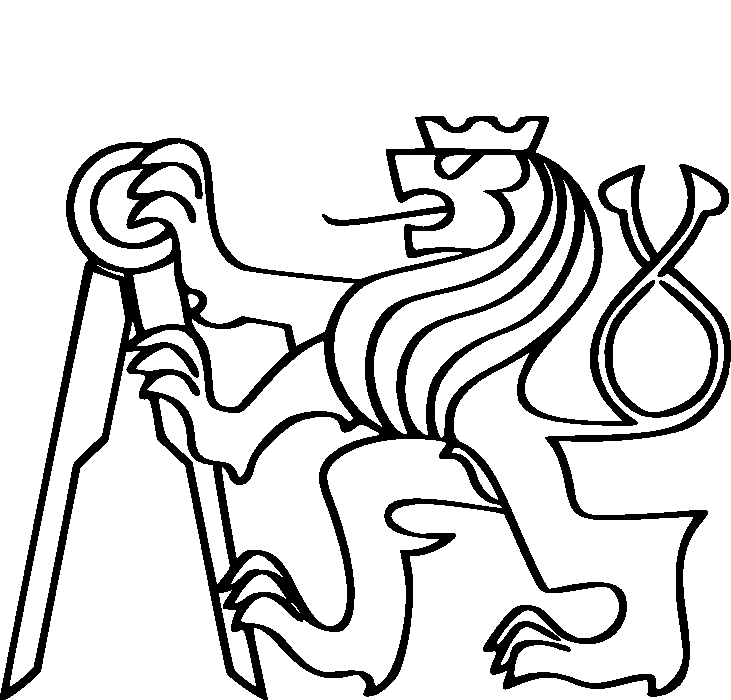
\includegraphics[scale=0.28]{../../_meta/cvut_standart.pdf}
\end{flushright}
\end{multicols}
\hrule
\vspace{0.5cm}

% ----------------------------------------------------------------------


% --- Tělo dokumentu ---------------------------------------------------

% Ocitovat markovu hlavičku
% Zeptat se na značky přístrojů

\setlength{\parindent}{0.5cm}

\section{Pracovní úkoly}
\begin{enumerate}
 \item \textbf{Domácí úkol:} Spočítejte, jakou vlastní a vyšší harmonické frekvence má struna napjatá zátěží 5 kg o délce 1 metr víte-li, že její lineární hustota je $\rho_l=0,0162\ \unit{kgm^{-1}}$.
 \item Do vzorce z předchozího úkolu dosaďte délku struny v praktiku a spočítejte totéž. Ověřte experimentálně pro prvních 10 rezonančních frekvencí. Z naměřených vyšších harmonických frekvencí zpětně dopočítejte lineární hustotu (použijte metodu nejmenších čtverců) a porovnejte s uvedenou konstantou. Dopočítejte rychlost šíření vlnění na struně. 
 \item Pro cca 10 různých frekvencí v rozsahu 2 až 6 kHz hledejte interferenční minima (nebo maxima) prodlužováním a zkracováním Quinckovy trubice. Vyneste do grafu závislost vlnové délky zvuku (prodloužení trubice) na frekvenci. Z naměřených údajů dopočítejte rychlost zvuku proložením naměřených hodnot s errorbary vhodnou funkcí.
 \item Najděte vlastní frekvence Helmholtzova dutinového rezonátoru. Vyneste závislost vlastní frekvence na objemu rezonátoru (změnu objemu rezonátoru provádějte vléváním vody). Vodu přilévejte po 50 ml a pouze do poloviny objemu. Pro hledání vlastní frekvence využijte Fourierovské frekvenční analýzy. Z naměřených hodnot určete rychlost zvuku proložením naměřených hodnot vhodnou funkcí.
\end{enumerate}

\section{Vypracování}

\subsection{Použité přístroje}
	Elektronický generátor kmitů s nastavitelnou frekvencí a amplitudou, generátor mechanického vlnění, kovová struna, závaží 5 kg, svinovací metr, vodiče, teploměr, Quinckova trubice, mikrofon, bateriový zesilovač, mikrofon se zesilovačem, reproduktor, osciloskop, Hemholtzův rezonátor (skleněná baňka), rozhraní COBRA, program PHYWE \cite{bib:phywe}, kádinka.

\subsection{Teoretický úvod}
	\subsubsection{Stojaté vlnění na struně}
		K určení lineární hustoty struny využíváme vzorce 
		
		\begin{equation}
		f_n = \frac{n}{2L} \sqrt{\frac{T}{\varrho}} = a \cdot n, \qquad a = \frac{1}{2L} \sqrt{\frac{T}{\varrho}},
		\label{eq:struna_uvod}
		\end{equation}		
		kde $f_n$ je frekvence $n$-tého módu, $L$ délka struny, $T=mg$ napětí na struně a $\varrho$ lineární hustota struny. Pomocí lineárního proložení závislosti $f_n(n)$ určíme parametr $a$ a z něj pak podle druhého vzorce lineární hustotu $\varrho$.
		Pro rychlost šíření platí vztahy 
		\begin{equation}
		v = f_n \lambda_n,\qquad \lambda_n = \frac{2L}{n},
		\label{eq:struna_rychlost}
		\end{equation}		
		
		kde $v$ je rychlost šíření vlny na struně, $L$ délka struny, $f_n$ frekvence n-tého módu a $\lambda_n$ jeho vlnová délka.		
		
	\subsubsection{Quinckova trubice}
		Quinckova trubice rozděluje zvuk do dvou různých větví, které spolu na výstupu interferují. Posunem jednoho z ramen můžeme měnit dráhu, kterou zvuk urazí v jedné z trubic, což mění fázi, se kterou interferují (a zároveň dochází k většímu tlumení amplitudy na delším rameni). Minimum naměřené intenzity nastává při podmínce 
		\begin{equation}
		\frac{\Delta \varphi}{2} = \frac{2n+1}{2} \cdot \pi \qquad n \in \mathbb{Z},
		\end{equation}
		což lze vyjádřit jako
		\begin{equation}
		d_n = \frac{2n+1}{2} \cdot \lambda \qquad n \in \mathbb{Z}.
		\end{equation}
		Vzdálenost mezi dvěma sousedními minimy odpovídá přesně polovině vlnové délky
		\begin{equation}
		\Delta d = d_{n+1} - d{n} = \frac{\lambda}{2}.
		\end{equation}
		Známe-li frekvenci vlnění $f$ (nastavujeme ji na generátoru), bude pro rychlost zvuku platit vztah
		\begin{equation}
		2\Delta d = \lambda = \frac{v}{f}.
		\label{eq:quinck}
		\end{equation}
		
	\subsubsection{Helmholtzovy rezonátory}
		Helmholtzův rezonátor v obecné podobě je pro nás systém sestávající se z okrouhlé dutiny a dlouhé trubice, která do ní vede. Platí-li předpoklad, že je délka trubice malá ve srovnání s vlnovou délkou zvuku, můžeme základní rezonanční frekvenci vyjádřit jako 
		\begin{equation}
		f = \frac{v}{2 \pi}\sqrt{\frac{\pi r^2}{(l + 1,4\cdot r)} \frac{1}{V}},
		\label{eq:helm}
		\end{equation}
		kde $v$ je rychlost zvuku, $l$ délka hrdla baňky, $r$ poloměr hrdla baňky a $V$ objem dutiny. Tento vzorec je však pouze přibližný a platí pouze, je-li objem hrdla mnohem menší, než objem dutiny. Proto pro menší objemy dutiny neplatí moc přesně.  Pro $1000$ml baňku jsou tyto hodnoty následující: $r = 0,0187$ m, $l = 0,07$ m, $V = 0,00103$ m$^3$.

\subsection{Postup měření}
	\subsubsection{Stojaté vlnění na struně}
		Nejdříve jsme sestavili aparaturu podle obrázku \ref{fig:s_struna} a pak měřili podle následujícího postupu:
		\begin{enumerate}
			\item Změříme délku struny od kladky po místo, kde je zaháknutá do generátoru mechanického vlnění.
			\item Na generátoru nastavíme předpokládanou frekvenci ($21,26$ Hz) prvního módu.
			\item Najdeme nejmenší možnou amplitudu, aby byly módy vidět.
			\item Ladíme jemněji frekvenci, dokud nenarazíme na další mód a zapíšeme jeho řád a frekvenci.
			\item Snížíme amplitudu, zdvojnásobíme frekvenci a znovu amplitudu zvýšíme.
			\item Kroky 4 a 5 opakujeme pro všechny hledané módy (6-10).   
		\end{enumerate}
		Při rozpoznávání módu jsme si museli dávat pozor na to, aby se amplituda kmitů periodicky neměnila. Pokud by se tak dělo, docházelo by k tzv. záznějům a bylo by nutné frekvenci dále ladit. 
		
		\begin{figure}
		 	\centering
		 	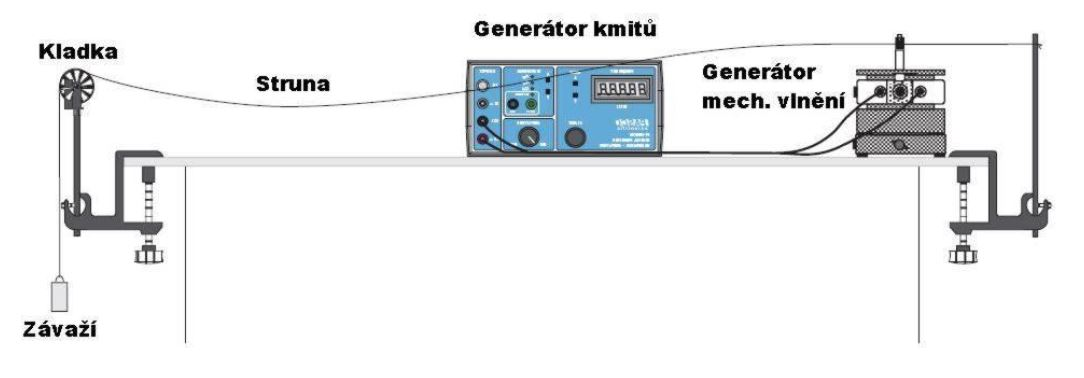
\includegraphics[width=.53\linewidth]{att/s_struna.jpg}
			\caption{Experimentální soustava pro pozorování stojatého vlnění na struně \cite{bib:zadani}.}
		    \label{fig:s_struna}
		\end{figure}
		
	\subsubsection{Quinckova trubice}
		Schéma Quinckovy trubice je vidět na obrázku \ref{fig:s_quinck}. Měření jsme prováděli pro 10 různých frekvencí a postupovali jsme následovně:
		\begin{enumerate}
			\item Začneme s nulovým rozdílem ramen (tedy $\Delta d=0$).
			\item Na generátoru nastavíme přibližně frekvenci (začínáme na $2,1$ kHz, s každým měřením o $0,4$ kHz zvýšíme) a ladíme ji tak, aby byl signál na osciloskopu stabilní (nejezdil z jedné strany na druhou).
			\item Příslušně nastavíme parametry osciloskopu.
			\item Měníme prodloužení jednoho z ramen, dokud nenarazíme na minimum. V té chvíli zapíšeme prodloužení $d$.
			\item Předchozí krok opakujeme, dokud neprodloužíme rameno maximálně.
		\end{enumerate}
		
		\begin{figure}
		 	\centering
		 	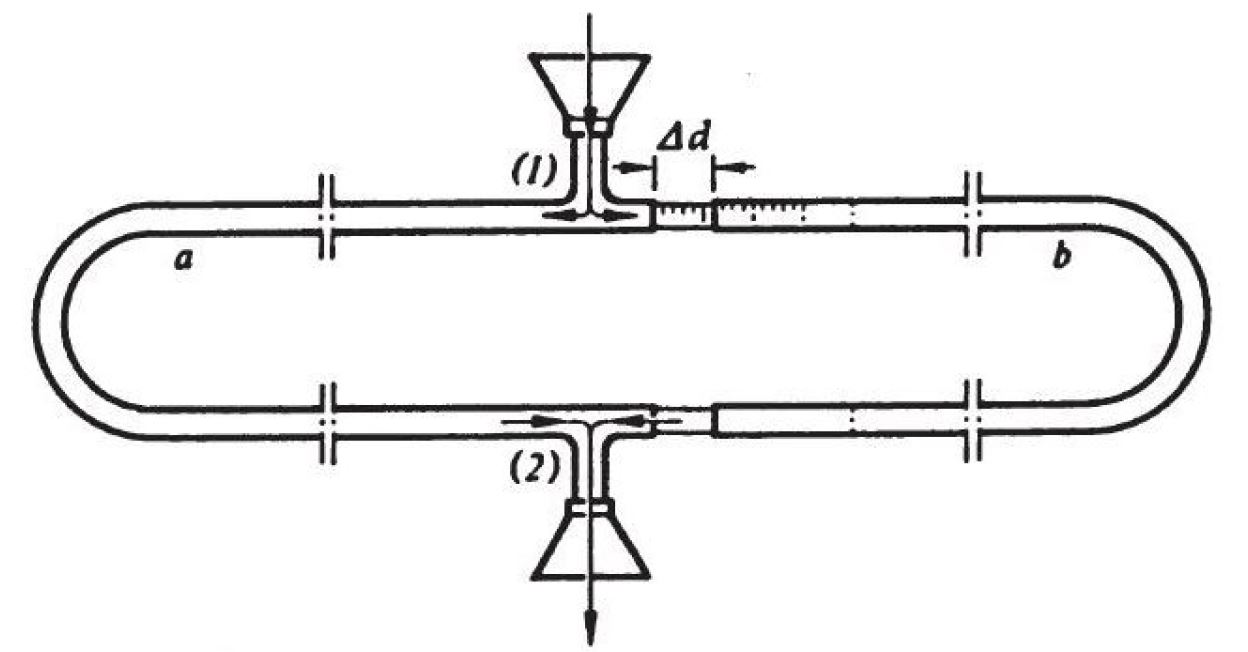
\includegraphics[width=.53\linewidth]{att/s_quinck.jpg}
			\caption{Schéma Quinckovy trubice \cite{bib:zadani}.}
		    \label{fig:s_quinck}
		\end{figure}		
	
	\subsubsection{Helmholtzovy rezonátory}
		Nastavili jsme aparaturu podle obrázku 9 z dokumentu \cite{bib:zadani}. Při měření jsme měnili frekvenci na generátoru a v programu PHYWE \cite{bib:phywe} studovali fourierovskou analýzu signálu. Nedbali jsme na první peak a hledali takovou frekvenci, při které byla amplituda druhého peaku maximální. Frekvenci jsme si v takový moment zapsali jako rezonanční a celý postup opakovali pro různý objem baňky. Vodu jsme dolévali po $50$ ml až do $0,5$ l a celé měření jsme provedli dvakrát za vystřídání členů skupiny.
		
\subsection{Naměřené hodnoty}
	\subsubsection{Stojaté vlnění na struně}
		\textbf{Domácí úkol:} podle vzorce \ref{eq:struna_uvod} jsme pro délku struny $L=1$ m, závaží o hmotnosti $m=5$ kg a lineární hustotu $\varrho=0,0162\ \unit{kgm^{-1}}$ spočítali
			\begin{equation}
			f_n = \frac{1}{2\cdot 1} \sqrt{\frac{5\cdot 9,81}{0,0162}}\ \dot{=}\ 27,51\ \unit{Hz}.
			\label{eq:struna_vypocet}
			\end{equation}		
		Pro délku struny v praktiku $L = (1,294 \pm 0,001)$ m jsme pak ze stejného vzorce dostali frekvenci $f_t = 21,26$ Hz.	
		 
		Naměřené hodnoty jsou uvedeny v tabulce \ref{tab:struna} a vyneseny do grafu \ref{fig:g_struna}, kde jsou lineárně proloženy. Z tohoto proložení dostáváme přímo hodnotu $a = (20,47 \pm 0,01)$. Pomocí druhé části vztahu \ref{eq:struna_uvod} poté odvodíme lineární hustotu i s chybou na
			\begin{equation}
			\varrho = (174,8 \pm 0,2)\ \cdot 10^{-4}\ \unit{kg/m}.
			\label{eq:struna_vysledky_1}
			\end{equation}
		Ze vztahu \ref{eq:struna_rychlost} poté dostáváme pro rychlost  
			\begin{equation}
			v = (52,98 \pm 0,03)\ \unit{m/s}.
			\label{eq:struna_vysledky_2}
			\end{equation}
					
		\begin{table}[h]
		\catcode`\-=12 % HAX na enable cline v českym bable
		\begin{center}
		\begin{tabular}{|r|r|r|}
		\hline
			$n$ [-]  &  $f$ [Hz]  &  $f_t$ [Hz]   \\\hline
		    $1$  &  $20,48$  &  $21,26$ \\\hline
		    $2$  &  $40,84$  &  $42,52$ \\\hline
		    $3$  &  $61,53$  &  $63,79$ \\\hline
		    $4$  &  $81,85$  &  $85,05$ \\\hline
		    $5$  &  $102,80$  &  $106,31$ \\\hline
		    $6$  &  $122,73$  &  $127,57$ \\\hline
		    $7$  &  $143,50$  &  $148,83$ \\\hline
		    $8$  &  $163,61$  &  $170,09$ \\\hline
		    $9$  &  $183,75$  &  $191,36$ \\\hline
		    $10$  &  $204,80$  &  $212,62$ \\\hline
		\end{tabular}
		\caption{Hledání vyšších harmonických frekvencí na struně. Počet kmiten je $n$, naměřená $n$-tá vyšší harmonická frekvence $f$, teoretická vyšší harmonická frekvence podle výpočtu z domácího úkolu $f_t$.}
		\label{tab:struna}
		\end{center}
		\end{table}
		
	\subsubsection{Quinckova trubice}
		Naměřené hodnoty jsou uvedeny v tabulce \ref{tab:quinck} a vyneseny do grafu \ref{fig:g_quinck}, kde jsou lineárně proloženy i s uvažováním chybových intervalů. Za použití vzorců \ref{eq:struna_uvod} a \ref{eq:struna_rychlost} tak z fitu získáváme velikost rychlosti zvuku jako 
			\begin{equation}
			v = (337 \pm 2)\ \unit{m/s}.
			\label{eq:quinck_vysledky}
			\end{equation}							
		
		\begin{table}[h]
		\catcode`\-=12 % HAX na enable cline v českym bable
		\begin{center}
		\begin{tabular}{|r|r|r|r|r|r|r|r|}
		\hline
			$f$ [Hz]  &  $\Delta d_1$ [cm]  &  $\Delta d_2$ [cm]  &  $\Delta d_3$ [cm]  &  $\overline{\Delta d}$ [cm]  &  $\sigma_{\Delta d}$ [cm]  &  $\lambda$ [cm]  &  $\sigma_{\lambda}$ [cm]   \\\hline
			    $2100$  &  $8,65$  &  $8,60$  &  $7,50$  &  $8,25$  &  $0,38$  &  $16,50$  &  $0,75$   \\\hline
			    $2500$  &  $6,60$  &  $7,00$  &  $7,20$  &  $6,93$  &  $0,18$  &  $13,87$  &  $0,35$   \\\hline
			    $2900$  &  $5,60$  &  $6,40$  &  $6,00$  &  $6,00$  &  $0,23$  &  $12,00$  &  $0,46$   \\\hline
			    $3300$  &  $5,00$  &  $4,70$  &  $6,10$  &  $5,27$  &  $0,43$  &  $10,53$  &  $0,85$   \\\hline
			    $3700$  &  $4,80$  &  $4,70$  &  $4,60$  &  $4,70$  &  $0,06$  &  $9,40$  &  $0,12$   \\\hline
			    $4100$  &  $4,25$  &  $4,05$  &  $4,40$  &  $4,23$  &  $0,10$  &  $8,47$  &  $0,20$   \\\hline
			    $4500$  &  $3,90$  &  $3,85$  &  $3,75$  &  $3,83$  &  $0,04$  &  $7,67$  &  $0,09$   \\\hline
			    $4900$  &  $3,50$  &  $3,50$  &  $3,55$  &  $3,52$  &  $0,02$  &  $7,03$  &  $0,03$   \\\hline
			    $5300$  &  $3,30$  &  $3,35$  &  $3,15$  &  $3,27$  &  $0,06$  &  $6,53$  &  $0,12$   \\\hline
			    $5700$  &  $3,10$  &  $2,90$  &  $3,20$  &  $3,07$  &  $0,09$  &  $6,13$  &  $0,18$   \\\hline
		\end{tabular}
		\caption{Měření intereference zvuku pomocí Quinckovy trubice. $f$ je frekvence nastavovaná na generátoru, $\Delta d_1, \Delta d_2, \Delta d_3$ naměřené hodnoty vzdáleností interferenčních minim, $\overline{\Delta d}$ jejich průměr, $\sigma_{\Delta d}$ chyba tohoto průměru, $\lambda$ z toho spočítaná vlnová délka a $\sigma_\lambda$ její chyba [\ref{eq:chyba_aritmetickeho_prumeru}].}
		\label{tab:quinck}
		\end{center}
		\end{table}	
		
	\subsubsection{Helmholtzovy rezonátory}
	Naměřené hodnoty jsou uvedeny v tabulce \ref{tab:helm} a vyneseny do grafu \ref{fig:g_helm}, kde jsou lineárně proloženy i s uvažováním chybových intervalů. Z tohoto proložení dostáváme přímo hodnotu $a = (5,57 \pm 0,02)$. Pomocí vztahu \ref{eq:helm} poté odvodíme rychlost zvuku jako
			\begin{equation}
			v = (327 \pm 1)\ \unit{m/s}.
			\label{eq:helm_vysledky}
			\end{equation}	 
		
		\begin{table}[h]
		\catcode`\-=12 % HAX na enable cline v českym bable
		\begin{center}
		\begin{tabular}{|r|r|r|r|r|}
		\hline
			$V$ [ml]  &  $f_1$ [Hz]  &  $f_2$ [Hz]  &  $\overline{f}$ [Hz]  &  $\sigma_f$ [Hz]   \\\hline
		    $1030$  &  $178,2$  &  $177,9$  &  $178,1$  &  $0,1$   \\\hline
		    $980$  &  $179,8$  &  $181,8$  &  $180,8$  &  $1,0$   \\\hline
		    $930$  &  $181,2$  &  $186,6$  &  $183,9$  &  $2,7$   \\\hline
		    $880$  &  $186,7$  &  $191,1$  &  $188,9$  &  $2,2$   \\\hline
		    $830$  &  $195,9$  &  $196,1$  &  $196,0$  &  $0,1$   \\\hline
		    $780$  &  $202,2$  &  $200,9$  &  $201,6$  &  $0,6$   \\\hline
		    $730$  &  $209,0$  &  $206,9$  &  $208,0$  &  $1,1$   \\\hline
		    $680$  &  $215,3$  &  $213,9$  &  $214,6$  &  $0,7$   \\\hline
		    $630$  &  $223,3$  &  $220,0$  &  $221,7$  &  $1,7$   \\\hline
		    $580$  &  $232,2$  &  $228,5$  &  $230,4$  &  $1,8$   \\\hline
		    $530$  &  $241,8$  &  $236,6$  &  $239,2$  &  $2,6$   \\\hline
		\end{tabular}
		\caption{Měření vlastních frekvencí Helmholtzova rezonátoru. $V$ je objem baňky, $f_1$ a $f_2$ naměřené frekvence, $\overline{f}$ jejich průměr a $\sigma_f$ chyba tohoto průměru [\ref{eq:chyba_aritmetickeho_prumeru}].}
		\label{tab:helm}
		\end{center}
		\end{table}
				
\subsection{Diskuse}	
	\subsubsection{Stojaté vlnění na struně}
		Od zhruba třetího módu dál začalo být přesnější určovat módy né hledáním uzlů a kmiten na struně, ale podle tónu struny. Bez metody poslechu by nejspíš nebylo možné určit více než 6 módů. Výsledky by se daly zpřesnit, pokud bychom brali menší ohled na okolní experimenty a využili plného rozsahu amplitudy. Tóny by pak byly hlasitější a zřetelnější a hodnoty by se daly určit s ještě větší přesností. Při malých amplitudách bylo také těžší určovat, kdy velikost výchylky kolísá s časem a dochází tak k záznějům. 
		
	\subsubsection{Quinckova trubice}
		Při teplotě $23\ \unit{^\circ C}$ je tabulková hodnota \cite{bib:tabulky} rychlosti zvuku ve vzduchu $345,5$ m/s. Nám se ji podařilo určit pomocí fitu na $v = (345,2 \pm 0,04)\ \unit{m/s}$, což je velmi přesná hodnota. Rozhodli jsme se měřit vzdálenosti interferenčních minim, jelikož se nám zdálo snažší je určovat, při volbě maxim by se ale přesnost příliš nezměnila. Absolutních minim signálu jsme nedosáhli nikdy, jelikož v místnosti nebyl dostatečný klid. Vzhledem k tomu, že se naše frekvence pohybovaly ve slyšitelném rozsahu, bylo třeba brát ohled na okolí a měření by šlo opět zpřesnit, pokud bychom využili celý rozsah nastavení amplitudy na generátoru. Při příštím měření by stálo za to měřit na úkor počtu frekvencí spíše více vzdáleností minim při každé z nich. 
		
	\subsubsection{Helmholtzovy rezonátory}
    	Tabulkovou hodnotu rychlosti zvuku ve vzduchu pro změřenou teplotu už jsme uváděli v diskusi metody s Quinckovou trubicí. Hodnota $v = (327 \pm 1)\ \unit{m/s}$ se od ní liší ještě více než předchozí měření. Tato nepřesnost byla zapříčiněna více faktory. Hlavním problémem bylo, že jsme provedli pouze dvě sady měření, což sice splňuje zadání, ale nezdá se to být dost. Chyby aritmetických průměrů tohoto měření nejsou směrodatné a statistická chyba i díky tomu vychází zanedbatelně malá. K dalším nepřesnostem vedlo, že mělo zobrazování peaků na počítači značnou setrvačnost a často bylo velmi těžké najít správnou frekvenci. Dále by se hodilo mít možnost přesně určit objem vody a vzduchu v baňce, jelikož nepřesnost každého dolití se zachovávala a chyby určování objemů dolité vody se tak sčítaly. Nepravděpodobným problémem je pak fakt, že byl mikrofon zapnutý (pravděpodobně od předchozího měření) už když jsme k úloze přišli. Je tedy možné, že v něm docházely baterie.
    	
\section{Závěr}
	Úspěšně jsme zjistili lineární hustotu struny a rychlost šíření vlny měněním frekvence při konstantním zatížení struny. Dále jsme určili přesněji a méně přesně rychlost zvuku pomocí metody Quinckovy trubice a Helmholtzova rezonátoru. 
	
\section {Použitá literatura}
% --- Literatura a reference -------------------------------------------
\begingroup
\renewcommand{\section}[2]{}

\begin{thebibliography}{9}
\bibitem{bib:zadani} Kolektiv KF, \emph{Návod k úloze: Akustika} [Online], [cit. \today] \newline 
http://praktikum.fjfi.cvut.cz/pluginfile.php/126/mod\_resource/content/4/akustika\_16\_10\_12.pdf

\bibitem{bib:repo} Kolektiv autorů, \emph{Repozitář zdrojů k praktiku} [Online] [cit. \today] \newline https://github.com/roesel/praktika

%\bibitem{bib:navody} Kolektiv KF, \emph{Návody k přístrojům} [Online], [cit. \today] \newline http://praktikum.fjfi.cvut.cz/documents/chybynav/navody-o.pdf

\bibitem{bib:phywe} Sploečnost PHYWE, \emph{Katalog produktů} [Online], [cit. \today] \newline 
http://www.phywe.com/448/Product-Catalogue.htm

\bibitem{bib:chyby} Kolektiv KF, \emph{Chyby měření} [Online], [cit. \today] \newline http://praktikum.fjfi.cvut.cz/documents/chybynav/chyby-o.pdf

\bibitem{bib:tabulky} J. Mikulčák a kol., Matematické, fyzikální a chemické tabulky \& vzorce. Prometheus,
Praha 2009.\newline
ISBN 978-80-7196-264-9

\end{thebibliography}
\endgroup
% ----------------------------------------------------------------------

\section{Přílohy}

\subsection{Domácí příprava}
	Domácí příprava je přiložena k protokolu.
\newpage
\subsection{Statistické zpracování dat}
	Pro statistické zpracování využíváme aritmetického průměru:
	\begin{equation} \label{eq:aritmeticky_prumer}
	\overline{x} = \frac{1}{n}\sum\limits_{i=1}^{n}x_i
	\end{equation}
	
	jehož chybu spočítáme jako 
	\begin{equation} \label{eq:chyba_aritmetickeho_prumeru}
	\sigma_0 = \sqrt{\frac{1}{n(n-1)} \sum\limits_{i=1}^{n}\left( x_i - \overline{x} \right)^2 },
	\end{equation}
	
	kde $ x_i $ jsou jednotlivé naměřené hodnoty, $ n $ je počet měření, $ \overline{x} $ aritmetický průměr a $ \sigma_0 $ jeho chyba \cite{bib:chyby}.
	
	Při nepřímém měření počítáme hodnotu s chybou dle následujících vztahů:
	\begin{equation}
	u = f(x, y, z, \ldots)
	\end{equation}
	\begin{displaymath}
	x = (\overline{x} \pm \sigma_x), \qquad
	y = (\overline{y} \pm \sigma_y), \qquad
	z = (\overline{z} \pm \sigma_z), \qquad
	\ldots,
	\end{displaymath}
	
	kde $ u $ je veličina, kterou určujeme nepřímo z měřených veličin $ x, y, z, \ldots $ 
	
	Pak
	\begin{displaymath}
	\overline{u} = f(\overline{x}, \overline{y}, \overline{z}, \ldots)
	\end{displaymath}
	\begin{equation}\label{eq:chyba_neprime_mereni}
	\sigma_u = \sqrt{\left( \frac{\partial f}{\partial x} \right)^2 \sigma^2_x + \left( \frac{\partial f}{\partial y} \right)^2 \sigma^2_y + \left( \frac{\partial f}{\partial z} \right)^2 \sigma^2_z + \ldots}
	\end{equation}
	\begin{displaymath}
	u = (\overline{u} \pm \sigma_ u),
	\end{displaymath}
\newpage
\subsection{Grafy}
	
	\begin{figure}[h]
	\begin{center}
	    %\vspace*{-1cm}
		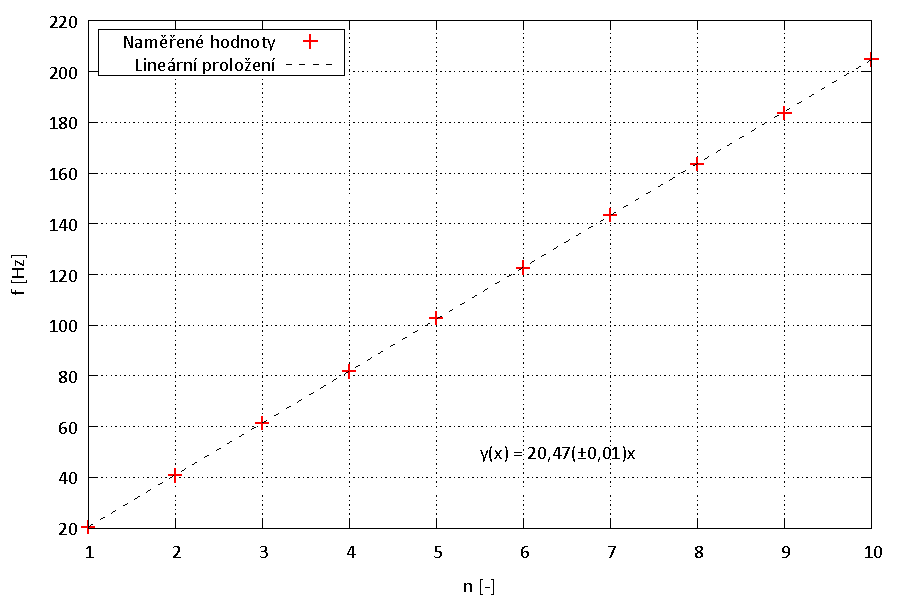
\includegraphics[width=\linewidth]{../gnuplot/9_aku_struna_out.pdf}
	    %\vspace*{-1cm}
		\caption{Graf měření frekvence $f$ kmitání struny v závislosti na počtu kmiten $n$. Proloženo lineárním fitem.}
		\label{fig:g_struna}
	\end{center}
	\end{figure}
	
	\begin{figure}[p]
	\begin{center}
		\vspace*{-1cm}
		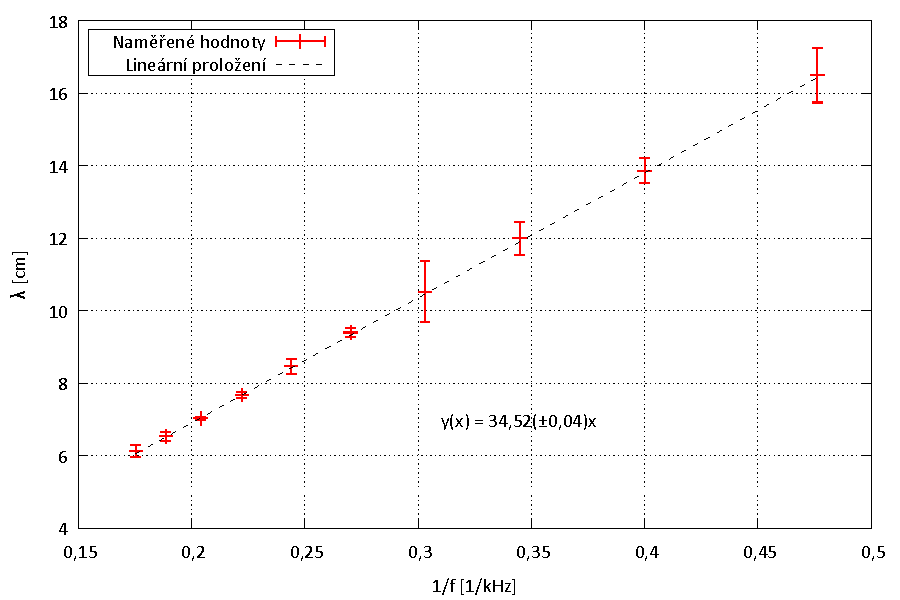
\includegraphics[width=\linewidth]{../gnuplot/9_aku_quinck_out.pdf}
		\vspace*{-1cm}    
		\caption{Graf měření vlnové délky zvuku $\lambda$ v závislosti na převrácené hodnotě frekvence $1/f$ a lineárního fitu.}
		\label{fig:g_quinck}
	\end{center}
	\end{figure}
	
	\begin{figure}[p]
	\begin{center}
	    \vspace*{-1cm}
	    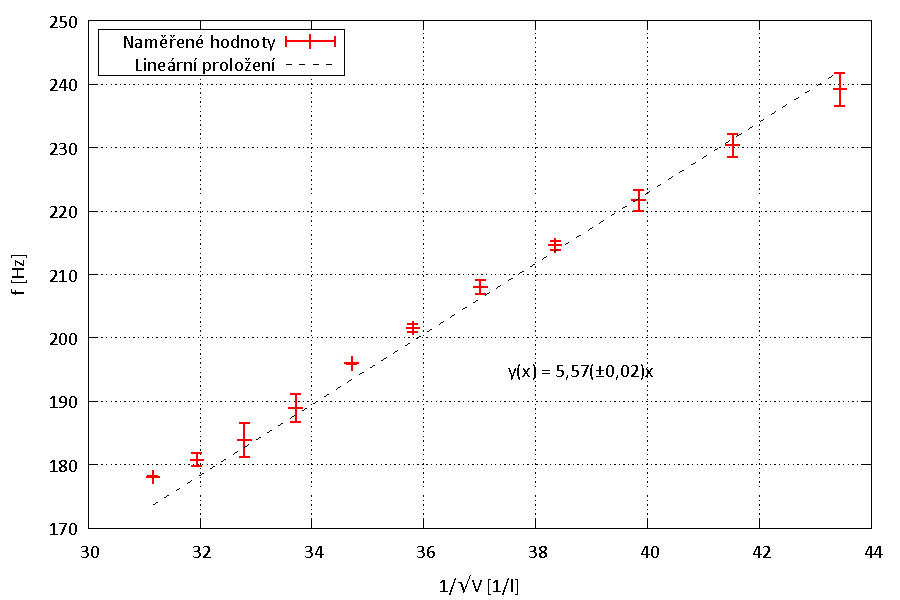
\includegraphics[width=\linewidth]{../gnuplot/9_aku_helm_out.pdf}
	    \vspace*{-1cm}    
		\caption{Graf měření frekvence v závislosti na převrácené hodnotě odmocniny z objemu $1/\sqrt(V)$ a lineárního fitu zohledňujícího chyby jednotlivých hodnot.}
		\label{fig:g_helm}
	\end{center}
	\end{figure}

% --- Konec dokumentu --------------------------------------------------


\end{document}

